\chapter{Orbitales moléculaires des molécules diatomiques}\label{ch:b2:diatomic-mos}

Versons du dioxygène liquide entre les pôles d'un aimant puissant~: il est attiré
sur le côté~; le diazote liquide, lui, tombe tout droit. La molécule de dioxygène porte des
électrons célibataires, qu'un champ magnétique attire. Son schéma de Lewis,
\ce{O=O} avec tous les électrons appariés, ne peut pas le dire. Les \omterm{def:b2:diatomic-mos:lcao}{orbitales moléculaires},
construites à partir des orbitales atomiques du chapitre précédent, placent chaque électron
d'une molécule sur un niveau qui lui est propre~: elles rendent compte du magnétisme du
dioxygène, de la force et de la longueur des liaisons, et des énergies nécessaires pour
ioniser les molécules --- et elles préparent la réactivité des
chapitres suivants.

\begin{recall}
\Cref{ch:b2:atomic-orbitals}~: les orbitales atomiques, leurs formes, leurs signes et leurs
énergies. Le volume de première année~: schémas de Lewis, liaisons $\sigma$ et $\pi$ comme
notions descriptives, hybridation et ses limites, électrons célibataires et
radicaux.
\end{recall}

\begin{omfigure}
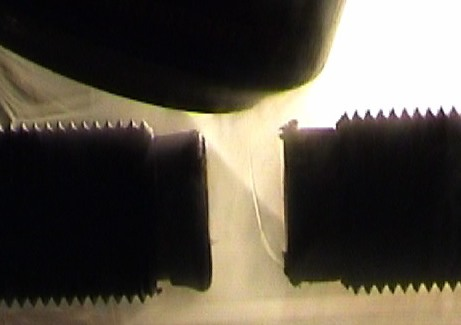
\includegraphics[width=0.42\linewidth]{images/book3/liquid-oxygen.jpg}

{\small Un mince filet de dioxygène liquide, qui tombe entre les pôles d'un aimant
puissant, est attiré vers eux et reste suspendu en pont~: la molécule est
\omterm{def:b2:diatomic-mos:magnetism}{paramagnétique}. (Photographie~: Pieter Kuiper, domaine public, Wikimedia Commons.)}
\end{omfigure}

\section{La méthode CLOA}

\begin{definition}[Orbitale moléculaire]\label{def:b2:diatomic-mos:lcao}
Une \emph{orbitale moléculaire}\index{orbitale moleculaire@orbitale moléculaire} est la \omterm{def:b2:atomic-orbitals:wavefunction}{fonction d'onde} d'un
électron dans une molécule, étendue à tous ses noyaux. Dans la méthode \emph{CLOA}\index{CLOA}
(combinaison linéaire d'orbitales atomiques), elle s'écrit comme une somme d'orbitales
atomiques des atomes, $\psi = \sum_i c_i\varphi_i$, avec des coefficients choisis pour
rendre l'énergie minimale.
\end{definition}

Pour deux atomes A et B apportant chacun une orbitale, $\psi = c_A\varphi_A + c_B\varphi_B$.
L'énergie d'un électron dans $\psi$, minimisée par rapport aux coefficients,
fait intervenir trois nombres.

\begin{definition}[Les intégrales de la méthode CLOA]\label{def:b2:diatomic-mos:integrals}
Pour deux orbitales atomiques réelles $\varphi_A$, $\varphi_B$ et l'opérateur énergie $\hat H$
d'un électron dans la molécule~:
\begin{itemize}
  \item l'\emph{intégrale de recouvrement}\index{integrale de recouvrement@intégrale de recouvrement} $S = \int\varphi_A\varphi_B\,dV$
        mesure à quel point les deux orbitales occupent la même région ($S = 1$ pour des
        orbitales identiques superposées)~;
  \item l'\emph{intégrale coulombienne}\index{integrale coulombienne@intégrale coulombienne} $\alpha_A = \int\varphi_A\hat
        H\varphi_A\,dV$ est l'énergie d'un électron dans $\varphi_A$ au sein de la molécule,
        proche de l'énergie de l'orbitale atomique~;
  \item l'\emph{intégrale de résonance}\index{integrale de resonance@intégrale de résonance} $\beta = \int\varphi_A\hat
        H\varphi_B\,dV$, négative, mesure le couplage des deux orbitales.
\end{itemize}
Les énergies $E$ des \omterm{def:b2:diatomic-mos:lcao}{orbitales moléculaires} sont les racines du \emph{déterminant
séculaire}\index{determinant seculaire@déterminant séculaire}
\[
  \begin{vmatrix} \alpha_A - E & \beta - ES \\ \beta - ES & \alpha_B - E \end{vmatrix} = 0 .
\]
\end{definition}

Le déterminant provient de la minimisation de $E = \int\psi\hat H\psi\,dV/\int\psi^2\,dV$
par rapport à $c_A$ et $c_B$~: les deux conditions $\partial E/\partial c_A =
\partial E/\partial c_B = 0$ forment un système linéaire homogène, qui n'a de solution
non nulle que si son déterminant s'annule. Cette étape variationnelle est admise
ici.

\begin{theorem}[Deux orbitales identiques]\label{thm:b2:diatomic-mos:homonuclear}
Pour $\alpha_A = \alpha_B = \alpha$, les deux \omterm{def:b2:diatomic-mos:lcao}{orbitales moléculaires} sont
\[
  E_+ = \frac{\alpha + \beta}{1 + S}, \quad \psi_+ = \frac{\varphi_A + \varphi_B}{\sqrt{2(1 + S)}} ;
  \qquad
  E_- = \frac{\alpha - \beta}{1 - S}, \quad \psi_- = \frac{\varphi_A - \varphi_B}{\sqrt{2(1 - S)}} .
\]
\end{theorem}

\begin{proof}
Le déterminant donne $(\alpha - E)^2 = (\beta - ES)^2$, donc $\alpha - E = \pm(\beta - ES)$.
Avec le signe plus, $E(1 + S) = \alpha + \beta$~; avec le signe moins, $E(1 - S) = \alpha
- \beta$. Reporté dans le système linéaire, $(\alpha - E)c_A + (\beta - ES)c_B = 0$ donne $c_B
= c_A$ pour $E_+$ et $c_B = -c_A$ pour $E_-$. Normalisation~: $\int(\varphi_A \pm
\varphi_B)^2\,dV = 2 \pm 2S$.
\end{proof}

\begin{definition}[Orbitales liantes et antiliantes]\label{def:b2:diatomic-mos:bonding}
Une \emph{orbitale liante}\index{orbitale liante} est située au-dessous des orbitales atomiques dont elle
est formée~: sa densité électronique s'accumule entre les noyaux. Une
\emph{orbitale antiliante}\index{orbitale antiliante} est située au-dessus d'elles et possède un
plan nodal entre les noyaux. Une \emph{orbitale non liante}\index{orbitale non liante}
conserve l'énergie de l'orbitale atomique, qui ne trouve aucun partenaire avec lequel
se combiner.
\end{definition}

\begin{proposition}[L'orbitale antiliante monte davantage]\label{prop:b2:diatomic-mos:asymmetry}
Pour $S > 0$, le niveau antiliant est élevé au-dessus de $\alpha$ de plus que le
niveau liant n'est abaissé au-dessous.
\end{proposition}

\begin{proof}
$E_+ - \alpha = (\beta - \alpha S)/(1 + S)$ et $E_- - \alpha = -(\beta - \alpha S)/(1 - S)$.
Le numérateur $\beta - \alpha S$ est négatif (le couplage domine), et $1 - S < 1
+ S$~: le second déplacement est le plus grand en valeur absolue.
\end{proof}

Avec deux électrons, comme dans \ce{H2}, tous deux occupent $\psi_+$ et la molécule est plus
stable que les atomes séparés. Avec quatre, comme dans \ce{He2}, deux doivent occuper $\psi_-$,
ce qui coûte plus que ce que $\psi_+$ fait gagner~: \ce{He2} n'est pas liée.

\begin{omfigure}
\begin{MOdiagram}[names, labels]
  \atom[H]{left}{ 1s = {0;up} }
  \atom[H]{right}{ 1s = {0;up} }
  \molecule[\ce{H2}]{ 1sMO = {.75;pair} }
\end{MOdiagram}
\hspace{1.5cm}
\begin{MOdiagram}[names, labels]
  \atom[He]{left}{ 1s = {0;pair} }
  \atom[He]{right}{ 1s = {0;pair} }
  \molecule[\ce{He2}]{ 1sMO = {.75;pair,pair} }
\end{MOdiagram}

{\small Diagrammes d'\omterm{def:b2:diatomic-mos:lcao}{orbitales moléculaires} de \ce{H2} (\omterm{def:b2:diatomic-mos:bond-order}{indice de liaison} 1) et de \ce{He2} (\omterm{def:b2:diatomic-mos:bond-order}{indice
de liaison} 0, molécule non liée). Chaque case est un niveau contenant au plus deux électrons de
spins opposés~; des tirets relient chaque \omterm{def:b2:diatomic-mos:lcao}{orbitale moléculaire} aux orbitales atomiques
dont elle est construite.}
\end{omfigure}

\section{Recouvrement et symétrie}

\begin{definition}[Orbitales $\sigma$ et $\pi$]\label{def:b2:diatomic-mos:sigma-pi}
Une \emph{orbitale $\sigma$}\index{orbitale sigma@orbitale $\sigma$} d'une molécule linéaire est inchangée par toute
rotation autour de l'axe moléculaire~: elle n'a aucun plan nodal contenant l'axe. Une
\emph{orbitale $\pi$}\index{orbitale pi@orbitale $\pi$} change de signe par une rotation de $180^\circ$ autour de
l'axe~: elle possède un plan nodal contenant l'axe. Un astérisque désigne les \omterm{def:b2:diatomic-mos:bonding}{orbitales
antiliantes} ($\sigma^*$, $\pi^*$).
\end{definition}

\begin{proposition}[Recouvrement nul par symétrie]\label{prop:b2:diatomic-mos:symmetry}
Deux orbitales dont l'une est symétrique et l'autre antisymétrique par rapport
à un plan contenant l'axe moléculaire ont un recouvrement nul et une \omterm{def:b2:diatomic-mos:integrals}{intégrale de
résonance} nulle~: elles ne se combinent pas.
\end{proposition}

\begin{proof}
La réflexion dans le plan laisse l'espace inchangé mais change le produit
$\varphi_A\varphi_B$ en son opposé au point symétrique~: les contributions des
deux moitiés de l'espace à $\int\varphi_A\varphi_B\,dV$ se compensent. Il en va de même pour
$\int\varphi_A\hat H\varphi_B\,dV$, puisque $\hat H$ a la symétrie de la molécule.
\end{proof}

Deux orbitales interagissent fortement lorsqu'elles ont la même symétrie (recouvrement
non nul), se recouvrent bien et sont proches en énergie. Une orbitale 1s d'un atome et une
$2\mathrm p_x$ de l'autre ($x$ perpendiculaire à l'axe) ne se combinent jamais~;
les orbitales $2\mathrm p_z$ (selon l'axe) donnent des orbitales $\sigma$~; les $2\mathrm p_x$ et
$2\mathrm p_y$ donnent deux paires d'orbitales $\pi$ de même énergie.

\begin{omfigure}
\begin{tikzpicture}[font=\small]
  % sigma 1s
  \pic at (0,0) {oms={0.85}}; \pic at (0.7,0) {oms={0.85}};
  \node at (0.35,-0.75) {$\sigma_{1s}$};
  \pic at (2.2,0) {oms={0.85}}; \pic at (2.9,0) {oms={-0.85}};
  \node at (2.55,-0.75) {$\sigma^*_{1s}$};
  % sigma 2p
  \pic at (4.6,0) {omp={-1}{0}}; \pic at (5.6,0) {omp={1}{0}};
  \node at (5.1,-0.75) {$\sigma_{2p}$};
  \pic at (7.4,0) {omp={-1}{0}}; \pic at (8.6,0) {omp={-1}{0}};
  \node at (8.0,-0.75) {$\sigma^*_{2p}$};
  % pi 2p
  \pic at (10.2,0) {omp={1}{90}}; \pic at (10.9,0) {omp={1}{90}};
  \node at (10.55,-0.95) {$\pi_{2p}$};
  \pic at (12.2,0) {omp={1}{90}}; \pic at (12.9,0) {omp={-1}{90}};
  \node at (12.55,-0.95) {$\pi^*_{2p}$};
  \draw[black!40, dashed] (-0.6,0) -- (13.4,0);
\end{tikzpicture}

{\small \omterm{def:b2:diatomic-mos:lcao}{Orbitales moléculaires} d'une molécule diatomique homonucléaire, schéma (l'axe
moléculaire est horizontal, en tirets). Les combinaisons en phase (liantes) rassemblent la
même couleur entre les noyaux~; les combinaisons en opposition de phase (antiliantes) placent un
plan nodal entre eux. Les orbitales $\sigma$ sont symétriques autour de l'axe~; chaque orbitale $\pi$
a l'axe dans son plan nodal.}
\end{omfigure}

\section{Les molécules diatomiques homonucléaires de la période 2}

Avec les orbitales 2s et 2p de deux atomes de la période 2, il se forme huit \omterm{def:b2:diatomic-mos:lcao}{orbitales moléculaires}~:
$\sigma_{2s}$, $\sigma^*_{2s}$, $\sigma_{2p}$, deux $\pi_{2p}$, deux $\pi^*_{2p}$,
$\sigma^*_{2p}$.

\begin{proposition}[Interaction s--p]\label{prop:b2:diatomic-mos:sp-mixing}
Pour \ce{O2} et \ce{F2}, l'ordre est $\sigma_{2s} < \sigma^*_{2s} < \sigma_{2p} < \pi_{2p} <
\pi^*_{2p} < \sigma^*_{2p}$. De \ce{Li2} à \ce{N2}, dont les niveaux 2s et 2p sont proches,
les orbitales $\sigma$ formées à partir de 2s et de $2\mathrm p_z$ se mélangent~: $\sigma_{2p}$ est repoussée
au-dessus de $\pi_{2p}$.
\end{proposition}

\begin{proof}[Argument]
Les orbitales $\sigma_{2s}$ et $\sigma_{2p}$ ont la même symétrie et peuvent se combiner
entre elles. Deux niveaux de même symétrie se repoussent (\cref{thm:b2:diatomic-mos:heteronuclear}
ci-dessous)~: $\sigma_{2s}$ descend, $\sigma_{2p}$ monte, d'autant plus qu'elles sont proches. L'écart
2s--2p augmente le long de la période~: l'effet est donc fort à gauche et faible pour
l'oxygène et le fluor. L'inversion entre l'azote et l'oxygène est admise d'après les
spectres photoélectroniques mesurés.
\end{proof}

\begin{definition}[Indice de liaison]\label{def:b2:diatomic-mos:bond-order}
L'\emph{indice de liaison}\index{indice de liaison} d'une molécule diatomique est $b = (n_b -
n_a)/2$, où $n_b$ et $n_a$ sont les nombres d'électrons dans les \omterm{def:b2:diatomic-mos:bonding}{orbitales liantes} et
antiliantes.
\end{definition}

\begin{proposition}[Indice de liaison et liaison]\label{prop:b2:diatomic-mos:bond-order}
Entre atomes d'un même couple d'éléments, un \omterm{def:b2:diatomic-mos:bond-order}{indice de liaison} plus élevé va de pair avec une liaison
plus courte et plus forte~; un \omterm{def:b2:diatomic-mos:bond-order}{indice de liaison} nul signifie l'absence de liaison.
\end{proposition}

\begin{proof}[Argument]
Chaque électron liant ajoute de la densité entre les noyaux et abaisse l'énergie~;
chaque électron antiliant en retire et élève l'énergie d'au moins autant
(\cref{prop:b2:diatomic-mos:asymmetry}). Le nombre net de paires liantes mesure
la liaison. La comparaison n'a de sens que pour des atomes semblables~: \ce{Li2} a un
\omterm{def:b2:diatomic-mos:bond-order}{indice de liaison} 1 comme \ce{F2}, mais ses orbitales 2s sont bien plus étendues.
\end{proof}

\begin{definition}[Paramagnétique et diamagnétique]\label{def:b2:diatomic-mos:magnetism}
Une substance est \emph{paramagnétique}\index{paramagnetique@paramagnétique} si ses molécules possèdent des
électrons célibataires~: elle est attirée dans un champ magnétique. Elle est
\emph{diamagnétique}\index{diamagnetique@diamagnétique} si tous ses électrons sont appariés~: elle est
faiblement repoussée hors du champ.
\end{definition}

\begin{omfigure}
\begin{MOdiagram}[names, labels, style=square, distance=4.2cm, labels-fs=\scriptsize]
  \atom[N]{left}{ 2s = {0;pair}, 2p = {3.5;up,up,up} }
  \atom[N]{right}{ 2s = {0;pair}, 2p = {3.5;up,up,up} }
  \molecule[\ce{N2}]{ 2sMO = {.7;pair,pair}, 2pMO = {0.4/2.5,1.4;pair,pair,pair} }
\end{MOdiagram}
\hfill
\begin{MOdiagram}[names, labels, style=square, distance=4.2cm, labels-fs=\scriptsize]
  \atom[O]{left}{ 2s = {0;pair}, 2p = {3.5;pair,up,up} }
  \atom[O]{right}{ 2s = {0;pair}, 2p = {3.5;pair,up,up} }
  \molecule[\ce{O2}]{ 2sMO = {.7;pair,pair}, 2pMO = {1.8,.8;pair,pair,pair,up,up} }
\end{MOdiagram}

{\small Diagrammes d'\omterm{def:b2:diatomic-mos:lcao}{orbitales moléculaires} de valence de \ce{N2} (à gauche, avec interaction s--p~:
$\sigma_{2p}$ au-dessus de $\pi_{2p}$) et de \ce{O2} (à droite). Diazote~: \omterm{def:b2:diatomic-mos:bond-order}{indice de liaison}
$(8 - 2)/2 = 3$, tous les électrons appariés. Dioxygène~: \omterm{def:b2:diatomic-mos:bond-order}{indice de liaison} $(8 - 4)/2 = 2$, avec deux
électrons célibataires dans les deux orbitales $\pi^*$ (règle de Hund)~: \ce{O2} est
\omterm{def:b2:diatomic-mos:magnetism}{paramagnétique}. Les diagrammes prennent $x$ comme axe moléculaire, d'où les étiquettes
$2\sigma_x$, $2\pi_y$, $2\pi_z$.}
\end{omfigure}

\begin{method}[Construire et remplir un diagramme d'OM]\label{met:b2:diatomic-mos:build-diagram}
\begin{enumerate}
  \item Placer les orbitales atomiques de valence de chaque atome à leur énergie, l'atome le plus
        électronégatif plus bas.
  \item Combiner les orbitales de même symétrie~: chaque paire donne une \omterm{def:b2:diatomic-mos:bonding}{orbitale liante}
        au-dessous et une \omterm{def:b2:diatomic-mos:bonding}{orbitale antiliante} au-dessus~; une orbitale sans partenaire reste
        non liante.
  \item Pour les molécules homonucléaires de la période 2, utiliser l'ordre avec $\sigma_{2p}$ au-dessus
        de $\pi_{2p}$ jusqu'à l'azote, au-dessous à partir de l'oxygène.
\end{enumerate}
\end{method}

\begin{method}[Lire un diagramme rempli]\label{met:b2:diatomic-mos:fill}
\begin{enumerate}
  \item Compter les électrons de valence (en ajouter un par charge négative, en retirer un
        par charge positive).
  \item Remplir à partir du bas, deux par orbitale, avec la règle de Hund pour les niveaux
        dégénérés.
  \item \omterm{def:b2:diatomic-mos:bond-order}{Indice de liaison} $(n_b - n_a)/2$~; les électrons célibataires donnent le paramagnétisme.
  \item Le niveau occupé le plus haut est le premier ionisé.
\end{enumerate}
\end{method}

\begin{omfigure}
\small
\renewcommand{\arraystretch}{1.15}
\begin{tabular}{lcccccc}
 & \ce{Li2} & \ce{C2} & \ce{N2} & \ce{O2} & \ce{F2} & \ce{NO} \\ \hline
électrons de valence & 2 & 8 & 10 & 12 & 14 & 11 \\
\omterm{def:b2:diatomic-mos:bond-order}{indice de liaison} & 1 & 2 & 3 & 2 & 1 & 2.5 \\
électrons célibataires & 0 & 0 & 0 & 2 & 0 & 1 \\
longueur de liaison $r_e$ (pm) & 267.3 & 124.3 & 109.8 & 120.8 & 141.2 & 115.1 \\
$D_0$ (\unit{eV}) & 1.04 & 6.15 & 9.76 & 5.12 & 1.60 & 6.51 \\
\end{tabular}

\smallskip
{\small Molécules diatomiques de la période 2~: \omterm{def:b2:diatomic-mos:bond-order}{indices de liaison} tirés des diagrammes d'OM~; longueurs de liaison
mesurées par spectroscopie, énergies de dissociation $D_0$ tirées des enthalpies de formation tabulées
à \qty{0}{K}, $D_0 = \Delta_f H_0(\mathrm A) + \Delta_f H_0(\mathrm B) - \Delta_f
H_0(\mathrm{AB})$.}
% ledger: re:Li2, re:C2, re:N2, re:O2, re:F2, re:NO, janafH0:Li, janafH0:Li2, janafH0:C, janafH0:C2, janafH0:N, janafH0:O, janafH0:F, janafH0:NO
\end{omfigure}

\section{Les molécules diatomiques hétéronucléaires}

\begin{theorem}[Deux orbitales d'énergies différentes]\label{thm:b2:diatomic-mos:heteronuclear}
Pour $\alpha_A > \alpha_B$ (B plus électronégatif), $S$ étant négligé, avec $\bar\alpha = (\alpha_A
+ \alpha_B)/2$ et $\Delta = \alpha_A - \alpha_B$~:
\[
  E_\mp = \bar\alpha \mp \sqrt{\Delta^2/4 + \beta^2} .
\]
L'\omterm{def:b2:diatomic-mos:bonding}{orbitale liante} (la plus basse) a son plus grand coefficient sur B, l'\omterm{def:b2:diatomic-mos:bonding}{orbitale antiliante}
sur A~; lorsque $\Delta \gg |\beta|$, $E_- \approx \alpha_B - \beta^2/\Delta$ et $E_+
\approx \alpha_A + \beta^2/\Delta$.
\end{theorem}

\begin{proof}
Avec $S = 0$, les énergies sont les valeurs propres de $\begin{pmatrix}\alpha_A & \beta \\
\beta & \alpha_B\end{pmatrix}$~: $(\alpha_A - E)(\alpha_B - E) = \beta^2$, dont les racines sont
$\bar\alpha \pm \sqrt{\Delta^2/4 + \beta^2}$. Pour la racine inférieure, $(\alpha_B - E_-)c_B = -\beta
c_A$~; $\alpha_B - E_- = \sqrt{\Delta^2/4 + \beta^2} - \Delta/2$ est inférieur à $|\beta|$, donc
$|c_A| < |c_B|$. Pour $\Delta \gg |\beta|$, $\sqrt{\Delta^2/4 + \beta^2} \approx \Delta/2 +
\beta^2/\Delta$.
\end{proof}

\begin{omfigure}
\begin{tikzpicture}
\begin{axis}[width=0.55\linewidth, height=6cm, xmin=0, xmax=8, ymin=-5, ymax=5,
  axis x line=bottom, axis y line=left, xlabel={$\Delta/|\beta|$}, ylabel={$E/|\beta|$},
  tick label style={font=\small}, label style={font=\small}]
\addplot[omThm, thick] table[x=d, y=Ehigh] {figdata/out/bachelor-2-two-level-a.dat};
\addplot[omDef, thick] table[x=d, y=Elow] {figdata/out/bachelor-2-two-level-a.dat};
\addplot[black!50, densely dotted] table[x=d, y=aA] {figdata/out/bachelor-2-two-level-a.dat};
\addplot[black!50, densely dotted] table[x=d, y=aB] {figdata/out/bachelor-2-two-level-a.dat};
\addplot[omThm, dashed] table[x=d, y=Phigh] {figdata/out/bachelor-2-two-level-a-pert.dat};
\addplot[omDef, dashed] table[x=d, y=Plow] {figdata/out/bachelor-2-two-level-a-pert.dat};
\node[font=\scriptsize, black!60, anchor=north west] at (axis cs:5.5,2.6) {$\alpha_A$};
\node[font=\scriptsize, black!60, anchor=south west] at (axis cs:5.5,-2.6) {$\alpha_B$};
\node[font=\scriptsize, omThm, anchor=south east] at (axis cs:3.2,2.2) {antiliante};
\node[font=\scriptsize, omDef, anchor=north east] at (axis cs:3.2,-2.2) {liante};
\end{axis}
\end{tikzpicture}

{\small Deux niveaux en interaction. Quand l'écart $\Delta$ entre les orbitales atomiques augmente,
les niveaux moléculaires (traits pleins) se rapprochent des niveaux atomiques (pointillés)~: la stabilisation
$\beta^2/\Delta$ de la limite perturbative (tirets) devient faible. Pour $\Delta = 0$, la
séparation vaut $2|\beta|$.}
\end{omfigure}

Dans le fluorure d'hydrogène, l'orbitale 1s de l'hydrogène rencontre les orbitales 2p, bien plus basses,
du fluor. Seule $2\mathrm p_z$, selon l'axe, a la bonne symétrie~: elle forme
une \omterm{def:b2:diatomic-mos:bonding}{orbitale liante} $\sigma$ développée surtout sur le fluor, et une $\sigma^*$ développée surtout sur
l'hydrogène. Les orbitales $2\mathrm p_x$ et $2\mathrm p_y$ du fluor restent
non liantes~: ce sont ses doublets non liants. La liaison est polarisée vers le fluor.

Le monoxyde de carbone possède les dix électrons de valence de \ce{N2} et un diagramme semblable,
mais les orbitales de l'oxygène sont plus basses. Ses \omterm{def:b2:diatomic-mos:bonding}{orbitales liantes} sont développées surtout sur l'oxygène~;
sa plus haute orbitale occupée, une orbitale $\sigma$ développée surtout sur le carbone, est un doublet non liant
du carbone. Le monoxyde de carbone se lie donc aux métaux par le carbone
(\cref{ch:b2:coordination-complexes}).

\begin{omfigure}
\begin{tikzpicture}[font=\small]
  % CO schematic: C left (higher), O right (lower)
  \pic (c2s) at (0,0.6) {omlevel={ud}{0.8}}; \node[left] at (-0.5,0.6) {2s};
  \pic (c2p1) at (-0.45,2.6) {omlevel={u}{0.4}}; \pic (c2p2) at (0,2.6) {omlevel={u}{0.4}}; \pic (c2p3) at (0.45,2.6) {omlevel={empty}{0.4}};
  \node[left] at (-0.75,2.6) {2p};
  \node at (0,-0.6) {C};
  \pic (o2s) at (6,-1.2) {omlevel={ud}{0.8}}; \node[right] at (6.5,-1.2) {2s};
  \pic (o2p1) at (5.55,1.4) {omlevel={ud}{0.4}}; \pic (o2p2) at (6,1.4) {omlevel={u}{0.4}}; \pic (o2p3) at (6.45,1.4) {omlevel={u}{0.4}};
  \node[right] at (6.75,1.4) {2p};
  \node at (6,-2.2) {O};
  % MOs
  \pic (m1) at (3,-1.8) {omlevel={ud}{0.8}};
  \pic (m2) at (3,-0.2) {omlevel={ud}{0.8}};
  \pic (m3a) at (2.75,0.9) {omlevel={ud}{0.45}}; \pic (m3b) at (3.25,0.9) {omlevel={ud}{0.45}};
  \pic (m4) at (3,1.9) {omlevel={ud}{0.8}};
  \pic (m5a) at (2.75,3.3) {omlevel={empty}{0.45}}; \pic (m5b) at (3.25,3.3) {omlevel={empty}{0.45}};
  \pic (m6) at (3,4.4) {omlevel={empty}{0.8}};
  \draw[omcorr, densely dashed] (c2s-r) -- (m1-l) (o2s-l) -- (m1-r);
  \draw[omcorr, densely dashed] (c2s-r) -- (m2-l) (o2s-l) -- (m2-r);
  \draw[omcorr, densely dashed] (c2p3-r) -- (m3a-l) (o2p1-l) -- (m3b-r);
  \draw[omcorr, densely dashed] (c2p3-r) -- (m4-l) (o2p1-l) -- (m4-r);
  \draw[omcorr, densely dashed] (c2p3-r) -- (m5a-l) (o2p1-l) -- (m5b-r);
  \draw[omcorr, densely dashed] (c2p3-r) -- (m6-l) (o2p1-l) -- (m6-r);
  \node[omsymlabel, below=0.17cm, inner sep=0.5pt] at (m1-c) {$\sigma$};
  \node[omsymlabel, below=0.17cm, inner sep=0.5pt] at (m2-c) {$\sigma$};
  \node[omsymlabel, below=0.17cm, inner sep=0.5pt] at (3,0.9) {$\pi$};
  \node[omsymlabel, below=0.24cm, inner sep=0.5pt] at (m4-c) {$\sigma$ (doublet de C)};
  \node[omsymlabel, below=0.05cm, inner sep=0.5pt] at (3,3.3) {$\pi^*$};
  \node[omsymlabel, below=0.05cm, inner sep=0.5pt] at (m6-c) {$\sigma^*$};
  \node at (3,-2.6) {CO};
\end{tikzpicture}

{\small Orbitales de valence du monoxyde de carbone, schéma~: les orbitales de l'oxygène sont
plus basses que celles du carbone. \omterm{def:b2:diatomic-mos:bond-order}{Indice de liaison} 3 comme dans \ce{N2}~; la plus haute orbitale
occupée est une orbitale $\sigma$ développée surtout sur le carbone, son doublet non liant.}
\end{omfigure}

\begin{history}[Hund et Mulliken]
\begin{minipage}[t]{0.27\linewidth}
\vspace{0pt}
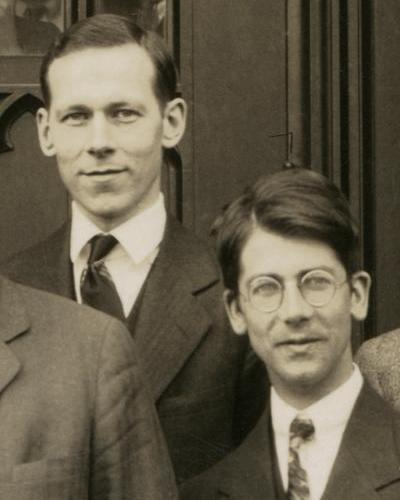
\includegraphics[width=\linewidth]{images/book3/mulliken-hund.jpg}
\end{minipage}\hfill
\begin{minipage}[t]{0.69\linewidth}
\vspace{0pt}
Entre 1926 et 1932, Friedrich Hund et Robert Mulliken interprétèrent les spectres
des molécules diatomiques en attribuant chaque électron à une orbitale de la molécule
entière, classée selon sa symétrie autour de l'axe. Les mots $\sigma$, $\pi$,
liante et antiliante, et les diagrammes d'orbitales de ce chapitre viennent de leurs
travaux~; Mulliken reçut le prix Nobel de chimie en 1966. La photographie montre
Mulliken (à gauche) et Hund à Chicago en 1929. (Photographie~: GFHund, CC BY 3.0,
Wikimedia Commons.)
\end{minipage}
\end{history}

\section{Ionisation et force de la liaison}

Arracher un électron à une \omterm{def:b2:diatomic-mos:bonding}{orbitale liante} affaiblit la liaison~; l'arracher à
une \omterm{def:b2:diatomic-mos:bonding}{orbitale antiliante} la renforce. Les énergies de dissociation des ions
se déduisent d'un cycle thermochimique~: pour $\mathrm{AB}^+ \to \mathrm A + \mathrm B^+$,
\[
  D_0(\mathrm{AB}^+) = D_0(\mathrm{AB}) + I(\mathrm B) - I(\mathrm{AB}) ,
\]
B étant l'atome de plus basse énergie d'ionisation.

\begin{example}[Les ions du diazote et du dioxygène]\label{ex:b2:diatomic-mos:ions}
\ce{N2} ($I = \qty{15.58}{eV}$) perd un électron liant~: $D_0(\ce{N2+}) = 9.76 + 14.53 -
15.58 = \qty{8.71}{eV}$, liaison plus faible que dans \ce{N2}. \ce{O2} ($I = \qty{12.07}{eV}$) perd un électron
$\pi^*$~: $D_0(\ce{O2+}) = 5.12 + 13.62 - 12.07 = \qty{6.66}{eV}$, liaison plus forte que dans \ce{O2},
en accord avec les \omterm{def:b2:diatomic-mos:bond-order}{indices de liaison} 2.5 et 2.5 contre 3 et 2.
% ledger: ie:N2, ie:N, ie:O2, ie:O, janafH0:N, janafH0:O
\end{example}

\section{Exercices}

\begin{exercise}[$\star$]\label{exo:b2:diatomic-mos:1}
Pour deux orbitales 1s de l'hydrogène, prendre $\alpha = \qty{-13.6}{eV}$, $\beta = \qty{-9.0}{eV}$ et
$S = 0.60$ (données de l'exercice). Calculer $E_+$ et $E_-$, puis l'énergie des deux
électrons de \ce{H2} comparée à celle de deux atomes séparés.
\end{exercise}

\begin{exercise}[$\star$]\label{exo:b2:diatomic-mos:2}
Donner les \omterm{def:b2:diatomic-mos:bond-order}{indices de liaison} de \ce{He2}, \ce{He2+}, \ce{Li2} et \ce{B2} (avec interaction
s--p).
\end{exercise}

\begin{exercise}[$\star$]\label{exo:b2:diatomic-mos:3}
Lesquelles des molécules \ce{B2}, \ce{C2}, \ce{N2}, \ce{O2}, \ce{F2} sont \omterm{def:b2:diatomic-mos:magnetism}{paramagnétiques}~?
\end{exercise}

\begin{exercise}[$\star$]\label{exo:b2:diatomic-mos:4}
L'axe moléculaire est $z$. Quelles paires parmi (1s, $2\mathrm p_z$), (1s,
$2\mathrm p_x$), ($2\mathrm p_x$, $2\mathrm p_x$), ($2\mathrm p_x$, $2\mathrm p_y$),
(2s, $2\mathrm p_z$) ont un recouvrement non nul~?
\end{exercise}

\begin{exercise}[$\star\star$]\label{exo:b2:diatomic-mos:5}
Prévoir si \ce{N2+} a une liaison plus longue ou plus courte que \ce{N2}, et vérifier à l'aide de
son énergie de dissociation calculée dans le chapitre.
\end{exercise}

\begin{exercise}[$\star\star$]\label{exo:b2:diatomic-mos:6}
Le monoxyde de carbone et \ce{N2} sont isoélectroniques. Expliquer pourquoi les \omterm{def:b2:diatomic-mos:bonding}{orbitales liantes} de
CO sont développées surtout sur l'oxygène et pourquoi sa plus haute orbitale occupée est un doublet non liant du
carbone.
\end{exercise}

\begin{exercise}[$\star\star$]\label{exo:b2:diatomic-mos:7}
Dans HF, quelles orbitales du fluor interagissent avec la 1s de l'hydrogène, et lesquelles restent
non liantes~? Tracer le diagramme.
\end{exercise}

\begin{exercise}[$\star\star$]\label{exo:b2:diatomic-mos:8}
Avec $\alpha_A = \qty{-10}{eV}$, $\alpha_B = \qty{-14}{eV}$ et $\beta = \qty{-3.0}{eV}$
(données de l'exercice, $S$ négligé), calculer les deux énergies et le poids $c_B^2$ de
l'\omterm{def:b2:diatomic-mos:bonding}{orbitale liante} sur B.
\end{exercise}

\begin{exercise}[$\star\star$]\label{exo:b2:diatomic-mos:9}
Avec l'interaction s--p, montrer que \ce{C2} a un \omterm{def:b2:diatomic-mos:bond-order}{indice de liaison} 2 formé de deux liaisons $\pi$ et d'aucune
liaison $\sigma_{2p}$.
\end{exercise}

\begin{exercise}[$\star\star\star$]\label{exo:b2:diatomic-mos:10}
Donner les \omterm{def:b2:diatomic-mos:bond-order}{indices de liaison} de NO et de \ce{NO+}. À partir de $D_0(\ce{NO}) = \qty{6.51}{eV}$, $I(\ce{NO}) =
\qty{9.26}{eV}$ et $I(\ce{O}) = \qty{13.62}{eV}$, calculer $D_0(\ce{NO+})$ pour $\ce{NO+} \to
\ce{N} + \ce{O+}$, et commenter.
\end{exercise}

\begin{exercise}[$\star\star\star$]\label{exo:b2:diatomic-mos:11}
Montrer que $E_+ + E_- = 2(\alpha - \beta S)/(1 - S^2)$, et que cette somme dépasse $2\alpha$ lorsque
$\beta < \alpha S < 0$. En déduire pourquoi deux orbitales pleines se repoussent (déstabilisation
à quatre électrons).
\end{exercise}

\begin{exercise}[$\star\star\star$]\label{exo:b2:diatomic-mos:12}
Classer \ce{O2+}, \ce{O2}, \ce{O2-}, \ce{O2^2-} par \omterm{def:b2:diatomic-mos:bond-order}{indice de liaison}, longueur de liaison et force de
liaison. Quel ion trouve-t-on dans le peroxyde d'hydrogène, et lequel dans le composé
jaune \ce{KO2}~?
\end{exercise}

\section{Problème~: le dioxygène et ses ions}

\begin{problem}[{Problème du week-end --- le diagramme d'orbitales moléculaires du dioxygène,
les indices de liaison et le magnétisme de ses ions, l'ionisation et la force de la
liaison, et les deux façons d'apparier les électrons $\pi^*$}]
\label{pb:b2:diatomic-mos:1}
Données~: $I(\ce{O}) = \qty{13.62}{eV}$, $I(\ce{O2}) = \qty{12.07}{eV}$, $I(\ce{N}) =
\qty{14.53}{eV}$, $I(\ce{N2}) = \qty{15.58}{eV}$~; $\Delta_f H_0$ à \qty{0}{K}
(\unit{kJ/mol})~: \ce{O} 246.79, \ce{N} 470.82~; $r_e$~: \ce{O2} \qty{120.8}{pm}, \ce{N2}
\qty{109.8}{pm}~; $1\ \unit{eV} = \qty{96.485}{kJ/mol}$.
% ledger: ie:O, ie:O2, ie:N, ie:N2, janafH0:O, janafH0:N, re:O2, re:N2

\medskip
\noindent\textbf{Partie I --- Le dioxygène.}
\begin{enumerate}
  \item Combien d'électrons de valence \ce{O2} possède-t-il~?
  \item Tracer son diagramme d'OM de valence (sans interaction s--p) et le remplir.
  \item Calculer son \omterm{def:b2:diatomic-mos:bond-order}{indice de liaison}.
  \item Combien d'électrons célibataires~? \ce{O2} est-il \omterm{def:b2:diatomic-mos:magnetism}{paramagnétique}~?
  \item Pourquoi le schéma de Lewis est-il ici en défaut~?
  \item Calculer $D_0(\ce{O2})$ en \unit{eV}.
\end{enumerate}

\medskip
\noindent\textbf{Partie II --- Les ions.}
\begin{enumerate}[resume]
  \item Donner la configuration et l'\omterm{def:b2:diatomic-mos:bond-order}{indice de liaison} de \ce{O2+}.
  \item Même question pour l'ion superoxyde \ce{O2-}.
  \item Même question pour l'ion peroxyde \ce{O2^2-}.
  \item Donner le nombre d'électrons célibataires de chaque ion.
  \item Classer \ce{O2+}, \ce{O2}, \ce{O2-}, \ce{O2^2-} par longueur de liaison prévue.
  \item Quel ion comporte une liaison simple O--O, comme le peroxyde d'hydrogène~?
  \item Lesquelles des quatre espèces sont \omterm{def:b2:diatomic-mos:magnetism}{paramagnétiques}~?
\end{enumerate}

\medskip
\noindent\textbf{Partie III --- L'ionisation.}
\begin{enumerate}[resume]
  \item De quelle orbitale part l'électron lorsqu'on ionise \ce{O2}~?
  \item Pourquoi $I(\ce{O2})$ est-elle inférieure à $I(\ce{O})$~?
  \item Montrer que $D_0(\ce{O2+}) = D_0(\ce{O2}) + I(\ce{O}) - I(\ce{O2})$ et la calculer.
  \item Comparer à $D_0(\ce{O2})$ et expliquer.
  \item Calculer de la même façon $D_0(\ce{N2})$ et $D_0(\ce{N2+})$.
  \item Pourquoi $I(\ce{N2})$ est-elle supérieure à $I(\ce{N})$~?
  \item Résumer~: quand l'ionisation renforce-t-elle une liaison~?
\end{enumerate}

\medskip
\noindent\textbf{Partie IV --- Les électrons $\pi^*$.}
\begin{enumerate}[resume]
  \item Dans l'état fondamental, les deux électrons $\pi^*$ occupent deux orbitales différentes avec
        des spins parallèles. Quelle règle l'impose~?
  \item Décrire un état dans lequel les deux occupent la même orbitale $\pi^*$.
  \item Pourquoi cet état est-il plus haut en énergie~?
  \item Quels sont son \omterm{def:b2:diatomic-mos:bond-order}{indice de liaison} et son magnétisme~?
  \item Donner l'\omterm{def:b2:diatomic-mos:bond-order}{indice de liaison} de \ce{O2+} et son énergie de dissociation.
\end{enumerate}
\end{problem}
